\noindent Each simulation generated six million 1332.492 keV gammas, indicative of a $^{60}$Co source.

\subsection{Quantification}
\noindent The following results are from the source located on the first floor in the central position as described in Table \ref{table:positions}.

\begin{figure}[!htb]
  \centering
  \includegraphics[width=\columnwidth]{images/5Det_Comparison_1fl_cen}
  \caption{Flux incident on detector plane}
  \label{fig:DetFlux1C}
\end{figure}

Fig. \ref{fig:DetFlux1C} shows the flux incident on the detector plane around the building. The flux is quantified into gross counts, full energy, partial energy, and scattering from the ground. There is a large amount of full energy depositions because the source location provides a clear line of sight to the detector.

\begin{figure}[!htb]
  \centering
  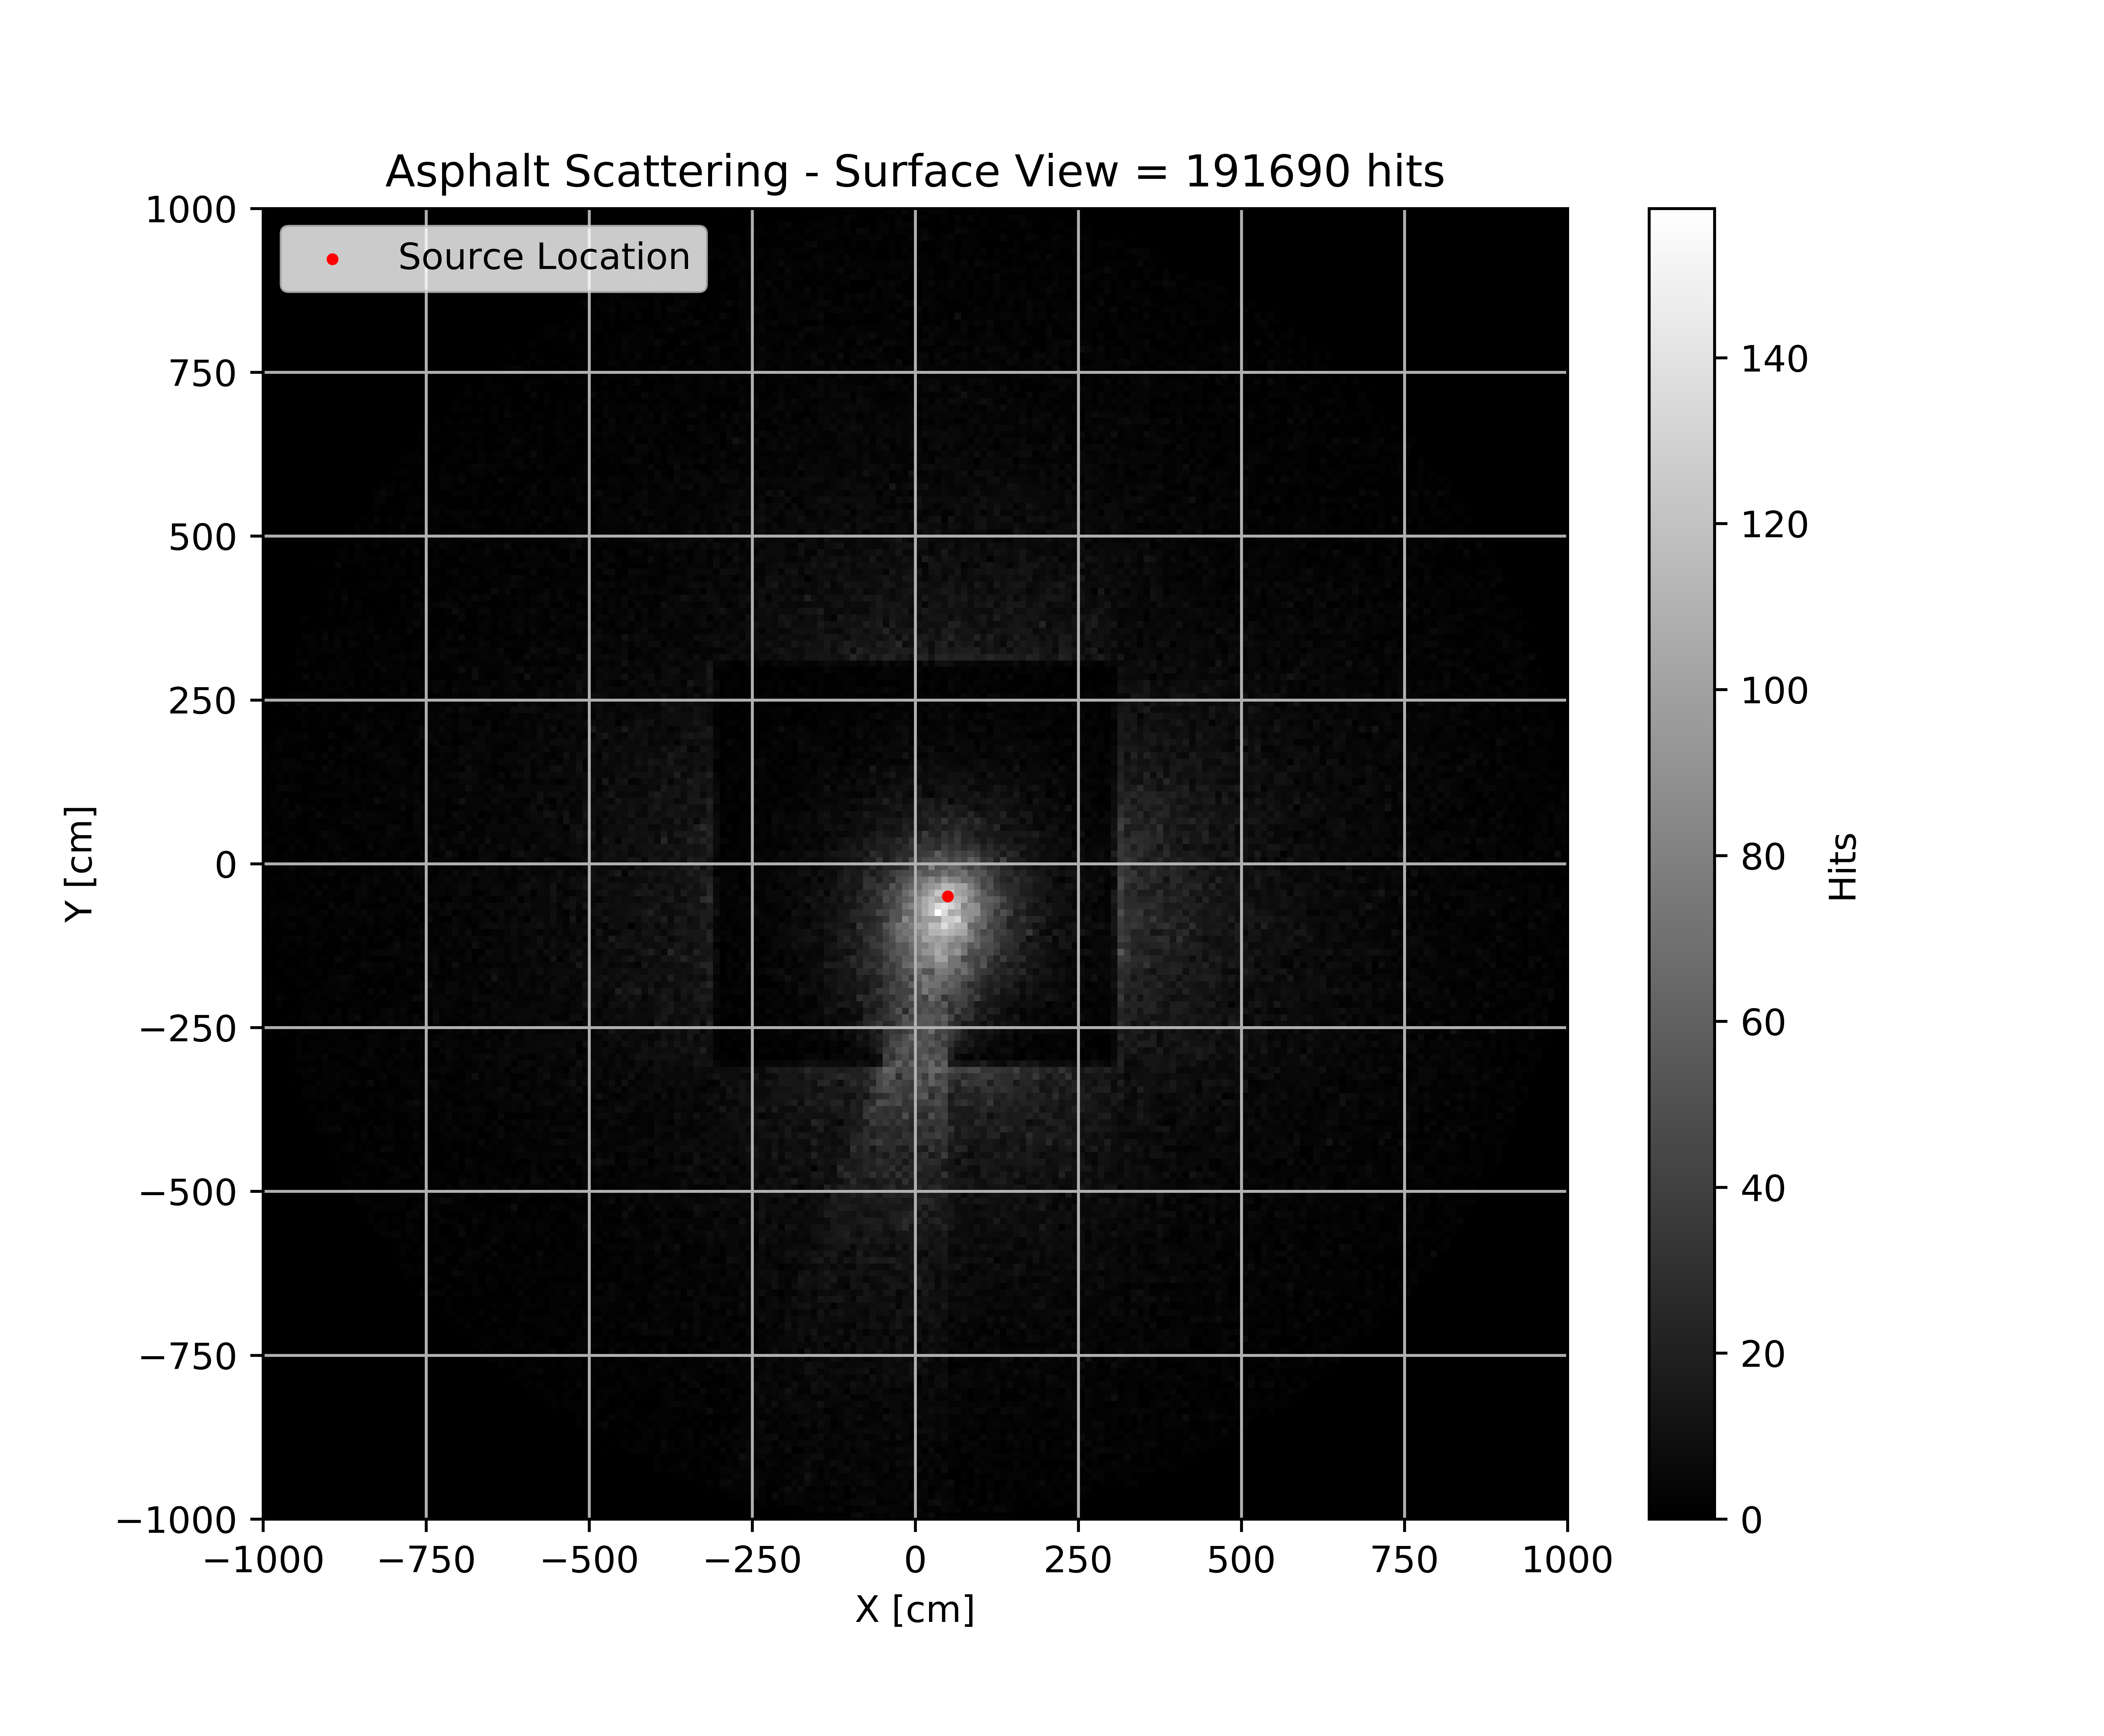
\includegraphics[width=\columnwidth]{images/10Asphalt_Scattered_1fl_cen}
  \caption{Ground flux due to gamma scattering off asphalt}
  \label{fig:AsScat1C}
\end{figure}

Fig. \ref{fig:AsScat1C} shows the ground flux due to gamma scattering off the asphalt. The unimpeded line of sight to the detector plane is clearly visible in this image.

\begin{figure}[!htb]
\begin{subfigure}[b]{0.55\textwidth}
   \centering
   \includegraphics[width=1\linewidth]{images/13Flux_South_Comparison_1fl_cen}
   \caption{}
   \label{fig:S1C}
\end{subfigure}
\begin{subfigure}[b]{0.55\textwidth}
   \centering
   \includegraphics[width=1\linewidth]{images/12Flux_North_Comparison_1fl_cen}
   \caption{}
   \label{fig:N1C}
\end{subfigure}
\caption{(a) The quantified flux as viewed from the South. (b) The quantified flux as viewed from the North.}
\end{figure}

\noindent This simulation clearly shows how an open door can assist in detection. Moreover, one would not expect to have more full energy hits than partial energy due to scattering when dealing with 10 cm concrete wall, however the open geometry gave the detector a large aperture with a direct line on sight.

\begin{figure}[!htb]
\begin{subfigure}[b]{0.55\textwidth}
   \centering
   \includegraphics[width=1\linewidth]{images/17_3D_Flux_Tot_1fl_cen}
   \caption{}
   \label{fig:3DT1C}
\end{subfigure}
\begin{subfigure}[b]{0.55\textwidth}
   \centering
   \includegraphics[width=1\linewidth]{images/17_3D_Flux_Full_1fl_cen}
   \caption{}
   \label{fig:3DF1C}
\end{subfigure}
\begin{subfigure}[b]{0.55\textwidth}
   \centering
   \includegraphics[width=1\linewidth]{images/17_3D_Flux_Part_1fl_cen}
   \caption{}
   \label{fig:3DP1C}
\end{subfigure}
\caption{(a) 3D quantified total flux as viewed from the Southeast. (b) 3D quantified full energy flux as viewed from the Southeast. (c) 3D quantified partial energy flux as viewed from the Southeast.}
\end{figure}

Figs. \ref{fig:3DT1C}, \ref{fig:3DF1C}, and \ref{fig:3DP1C} show 3D depictions of the quantified flux. Fig. \ref{fig:3DF1C} has no ground plane because all gammas traced back to the asphalt were scattering events that resulted in a loss of energy.

\subsection{Localization}
\noindent The following results are from the source located on the second floor in position closest to the wall as described in Table \ref{table:positions}.

\begin{figure}[!htb]
\begin{subfigure}[b]{0.5\textwidth}
   \centering
   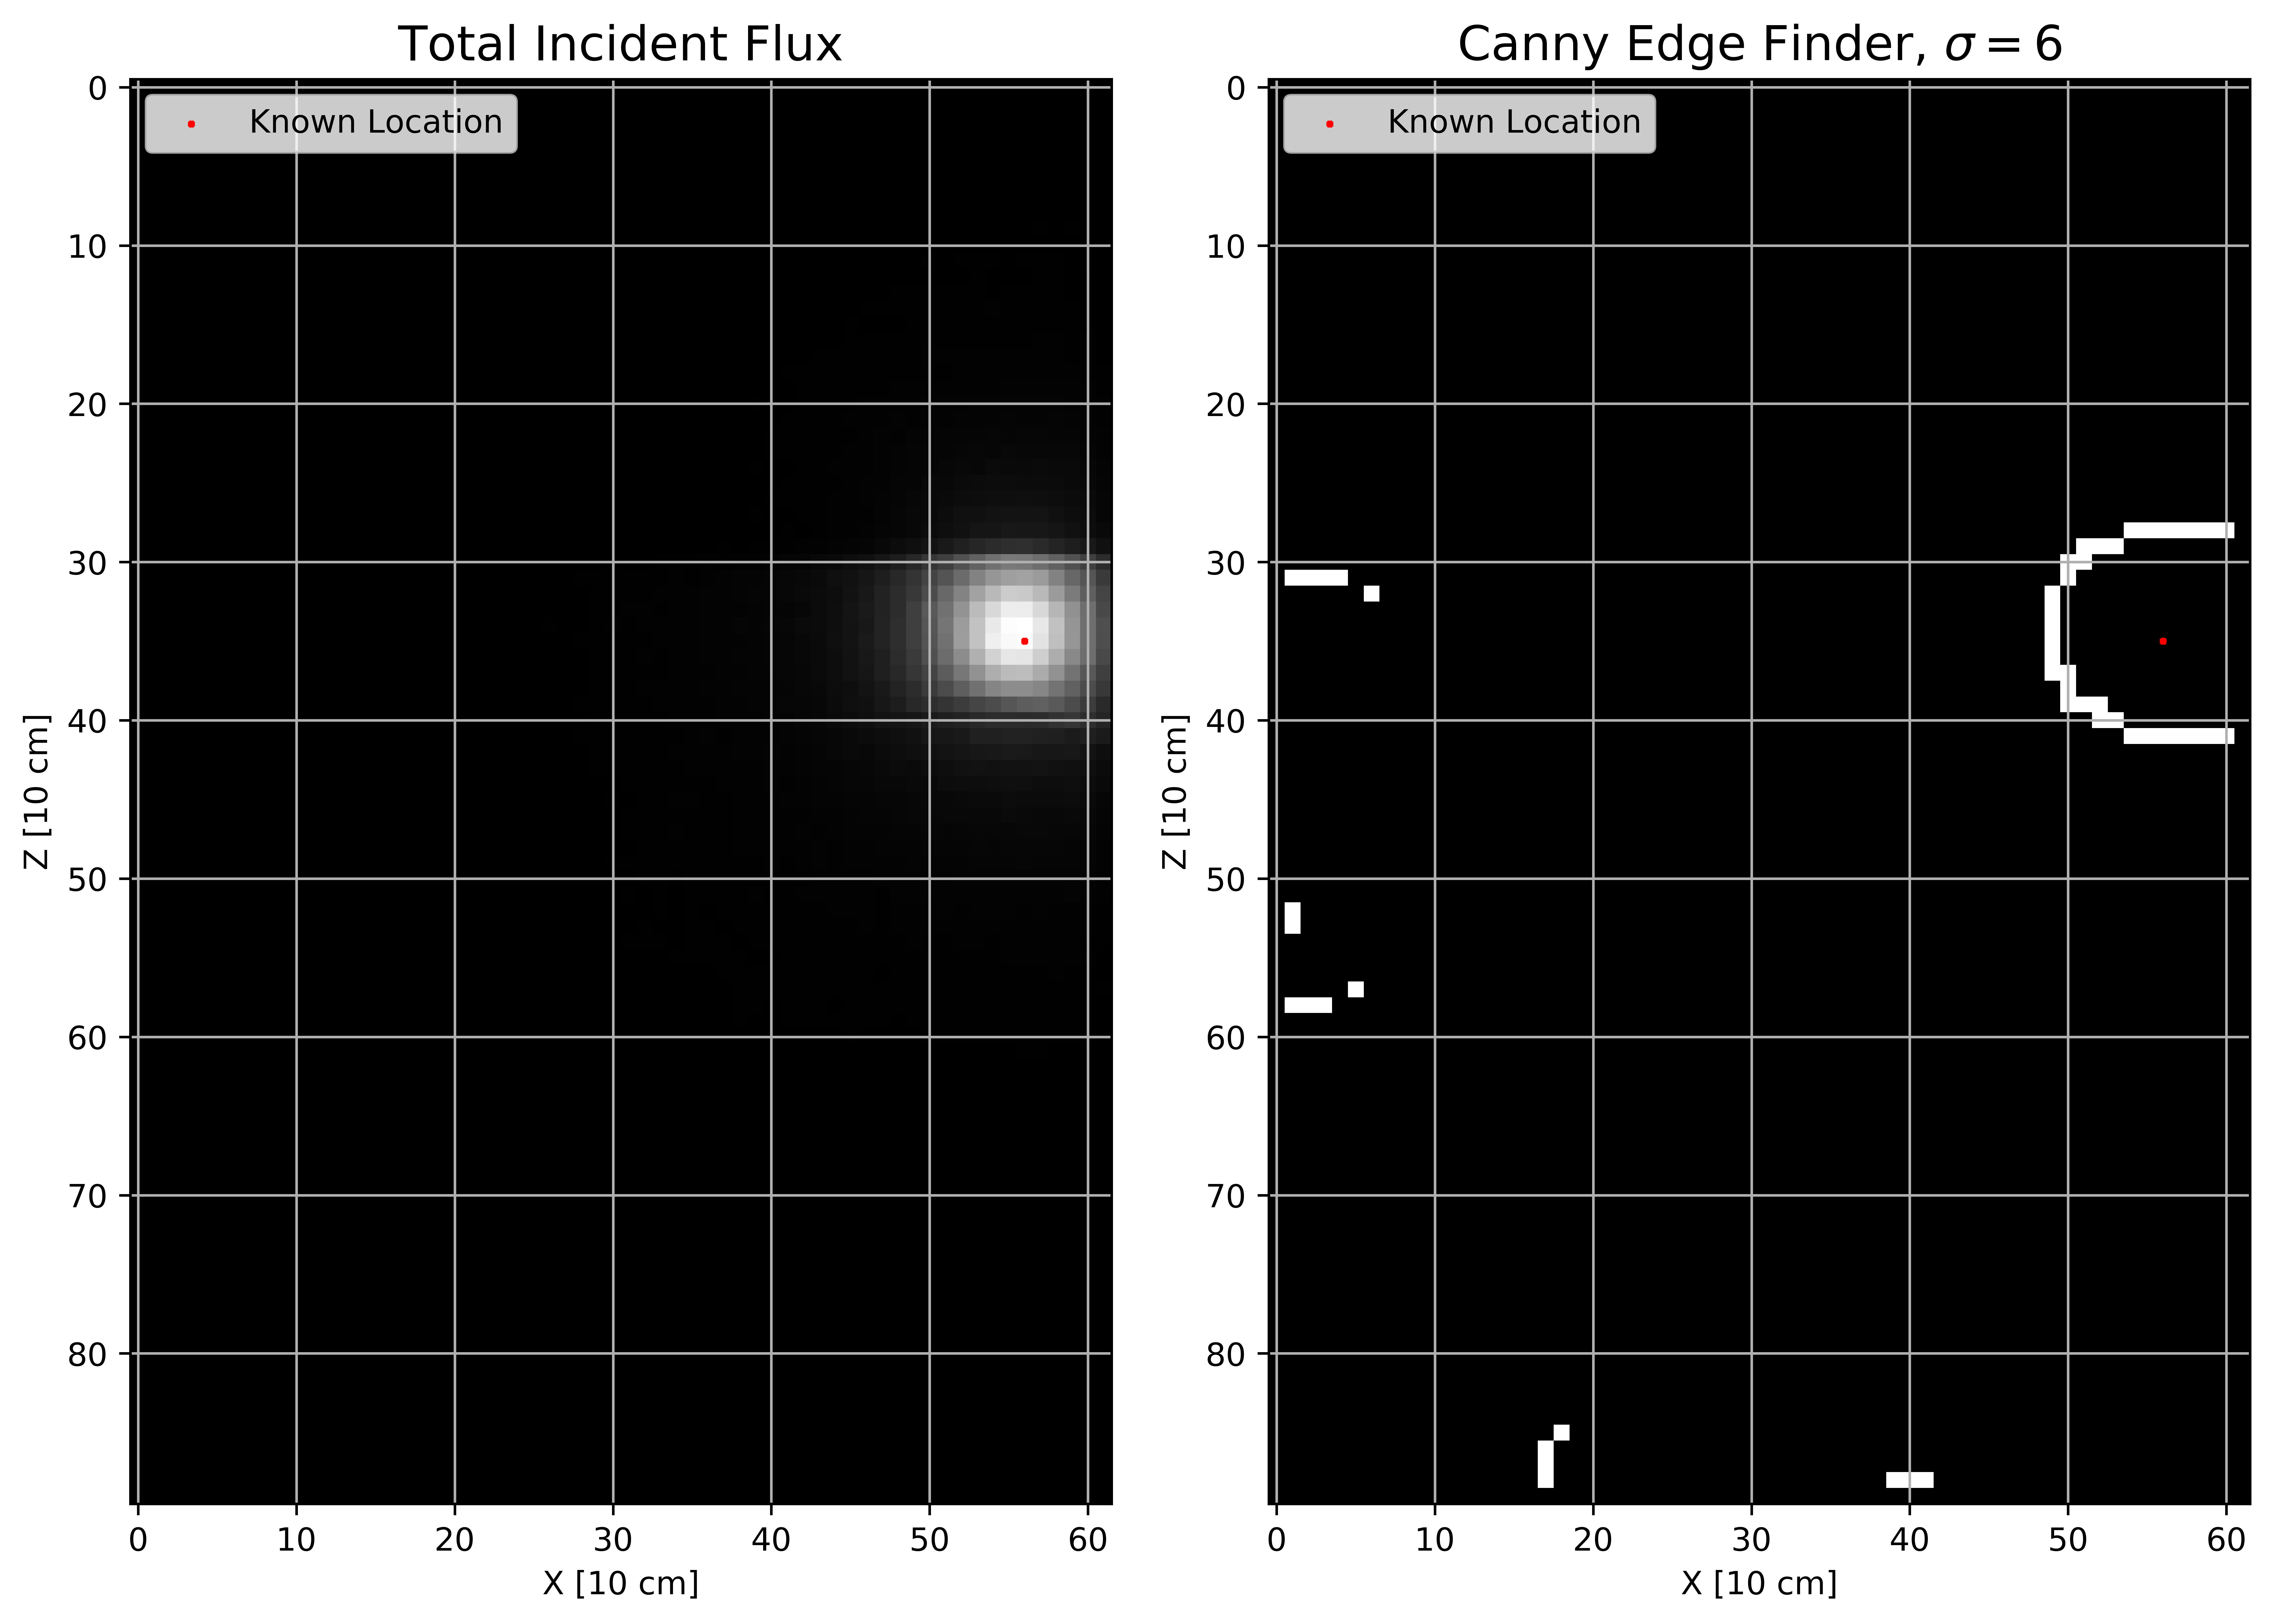
\includegraphics[width=1\linewidth]{images/1Canny_Total_2fl_Wall_S}
   \caption{}
   \label{fig:Can2FTotS}
\end{subfigure}
\begin{subfigure}[b]{0.5\textwidth}
   \centering
   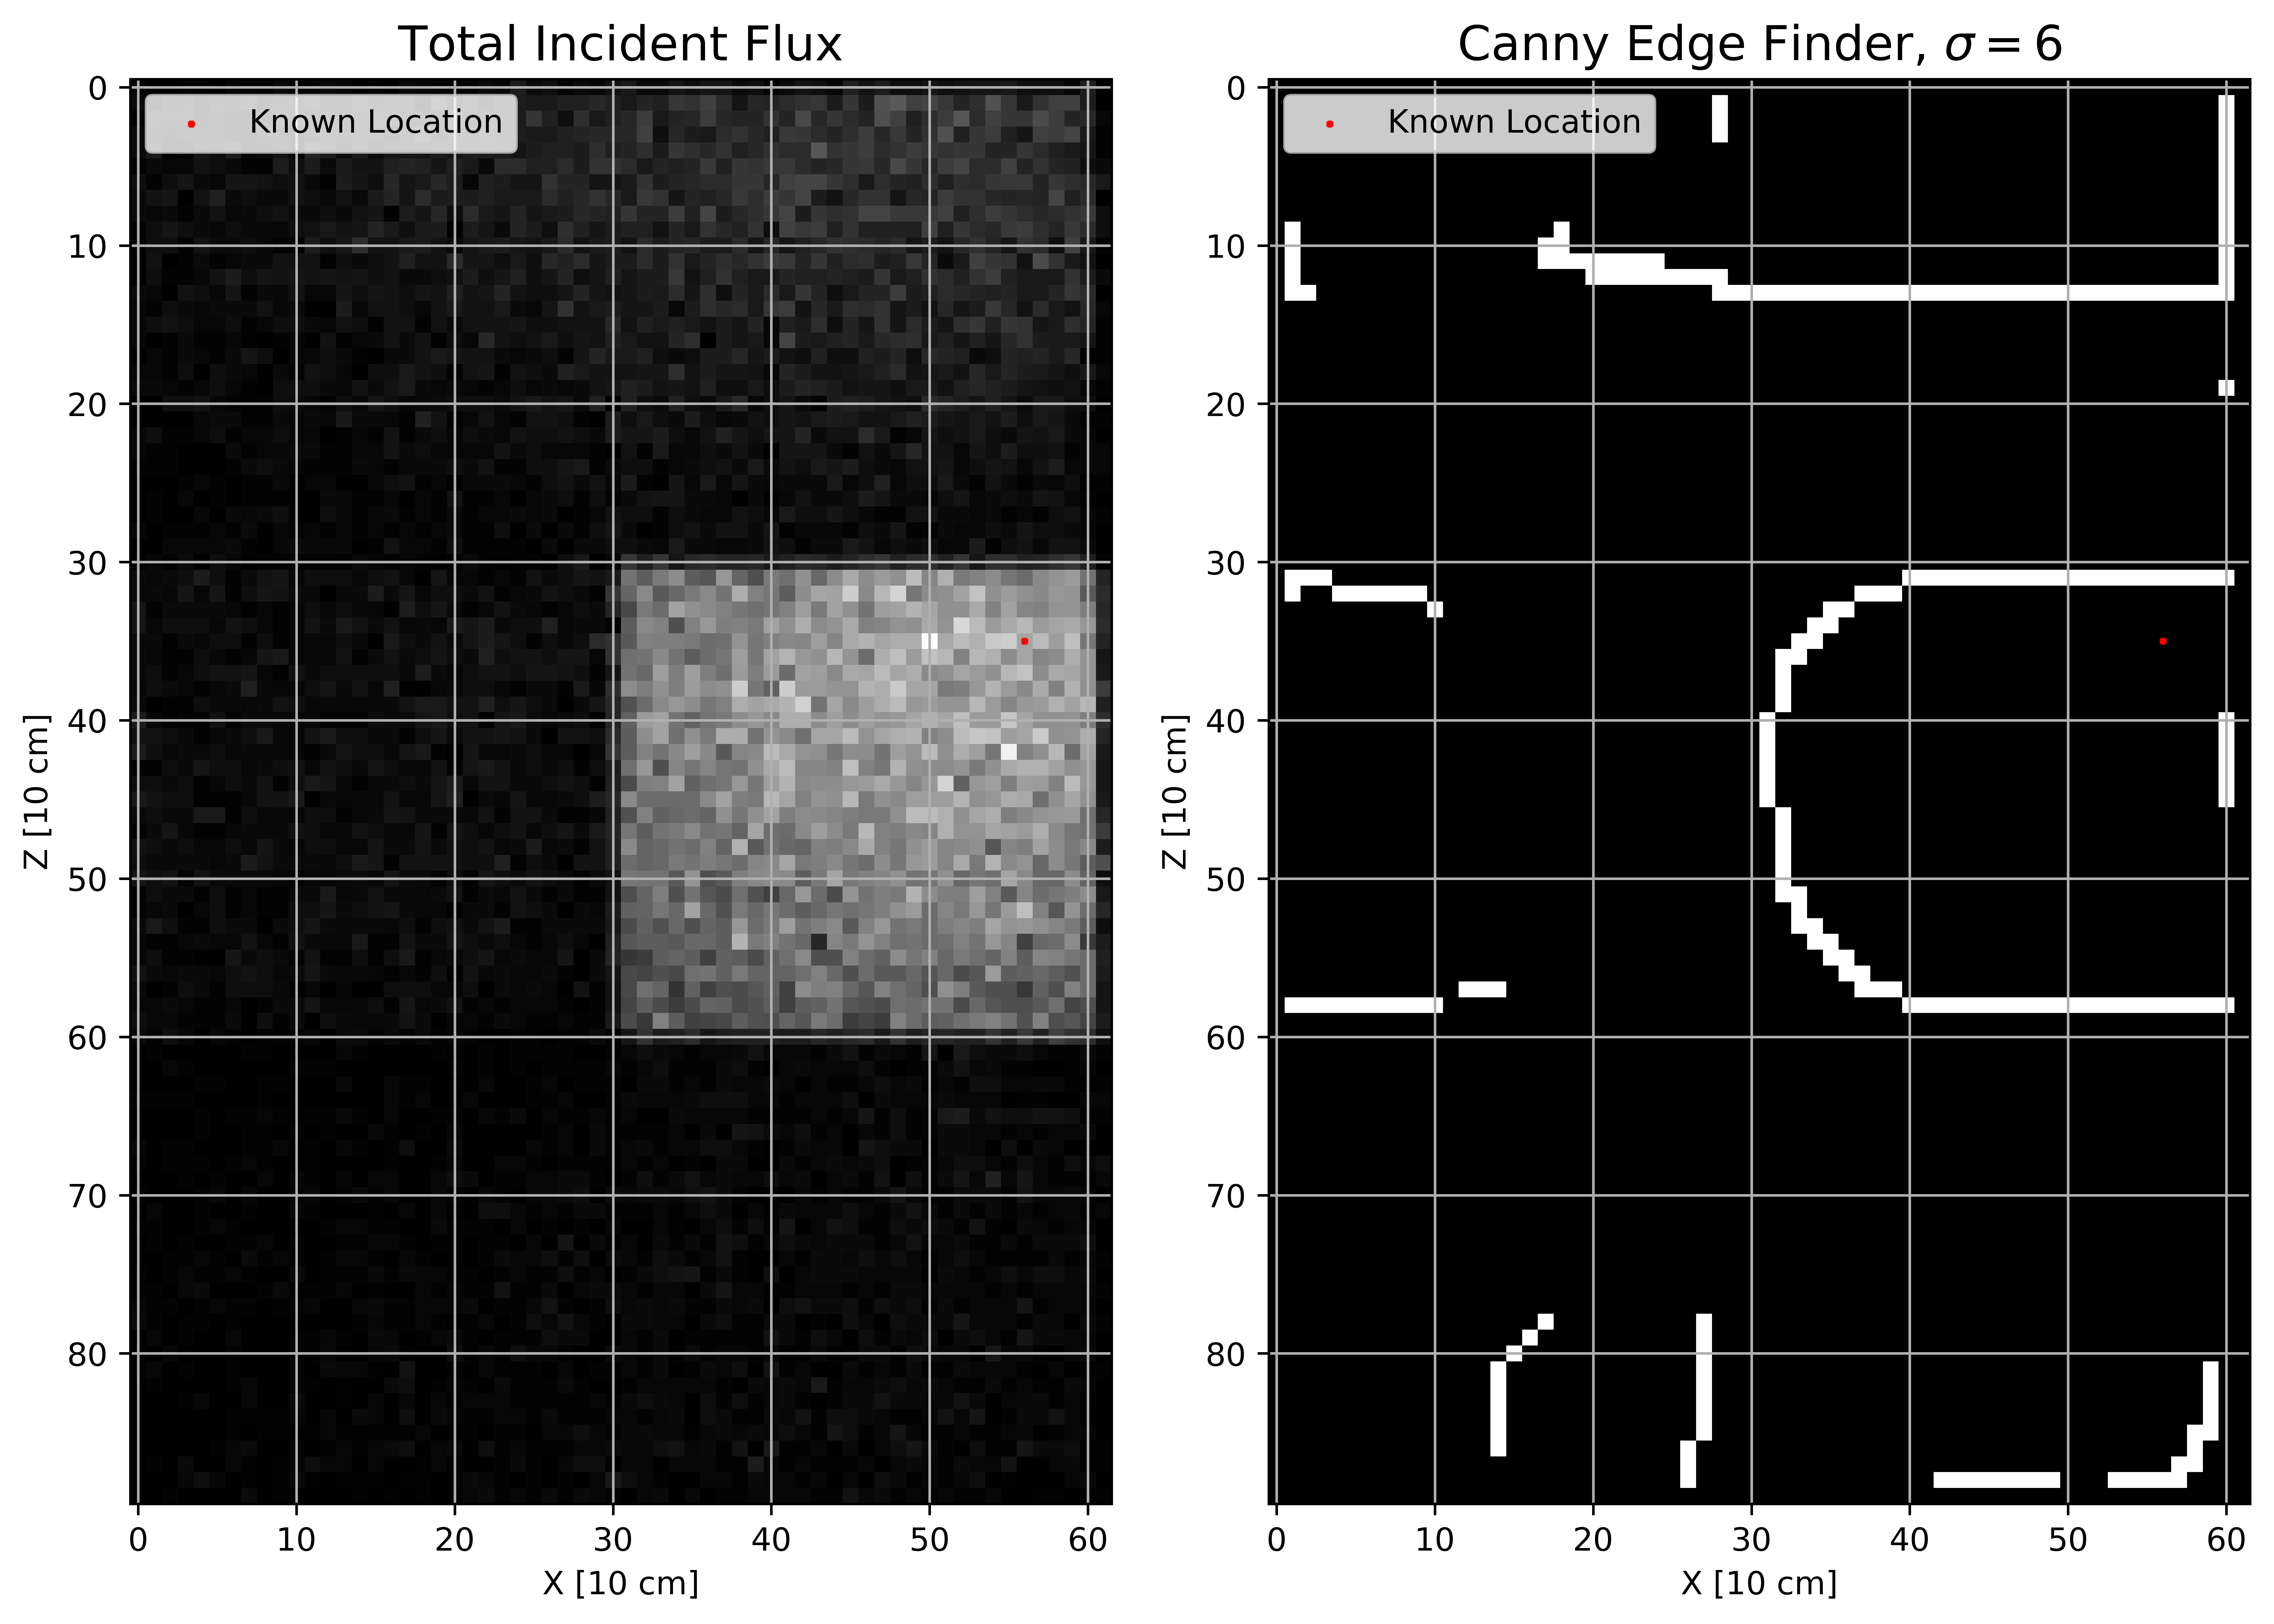
\includegraphics[width=1\linewidth]{images/1Canny_Total_2fl_Wall_N}
   \caption{}
   \label{fig:Can2FTotN}
\end{subfigure}
\caption{(a) The quantified total flux and 6$\sigma$ Canny filter as viewed from the South. (b) The quantified total flux and 6$\sigma$ Canny filter as viewed from the North.}
\end{figure}

\noindent Figs. \ref{fig:Can2FTotS} and \ref{fig:Can2FTotN} show the first step of localization, implementing a Canny edge finder. Fig. \ref{fig:Can2FTotS} also demonstrates how the closer a source is to a surface, the more concentrated the flux distribution, which can lead to more precise localization. Fig. \ref{fig:Can2FTotN} demonstrates how a building's construction, in this case internal walls, can assist in localization by limiting excess gamma transmission.

\begin{figure}[!htb]
\begin{subfigure}[b]{0.15\textwidth}
   \centering
   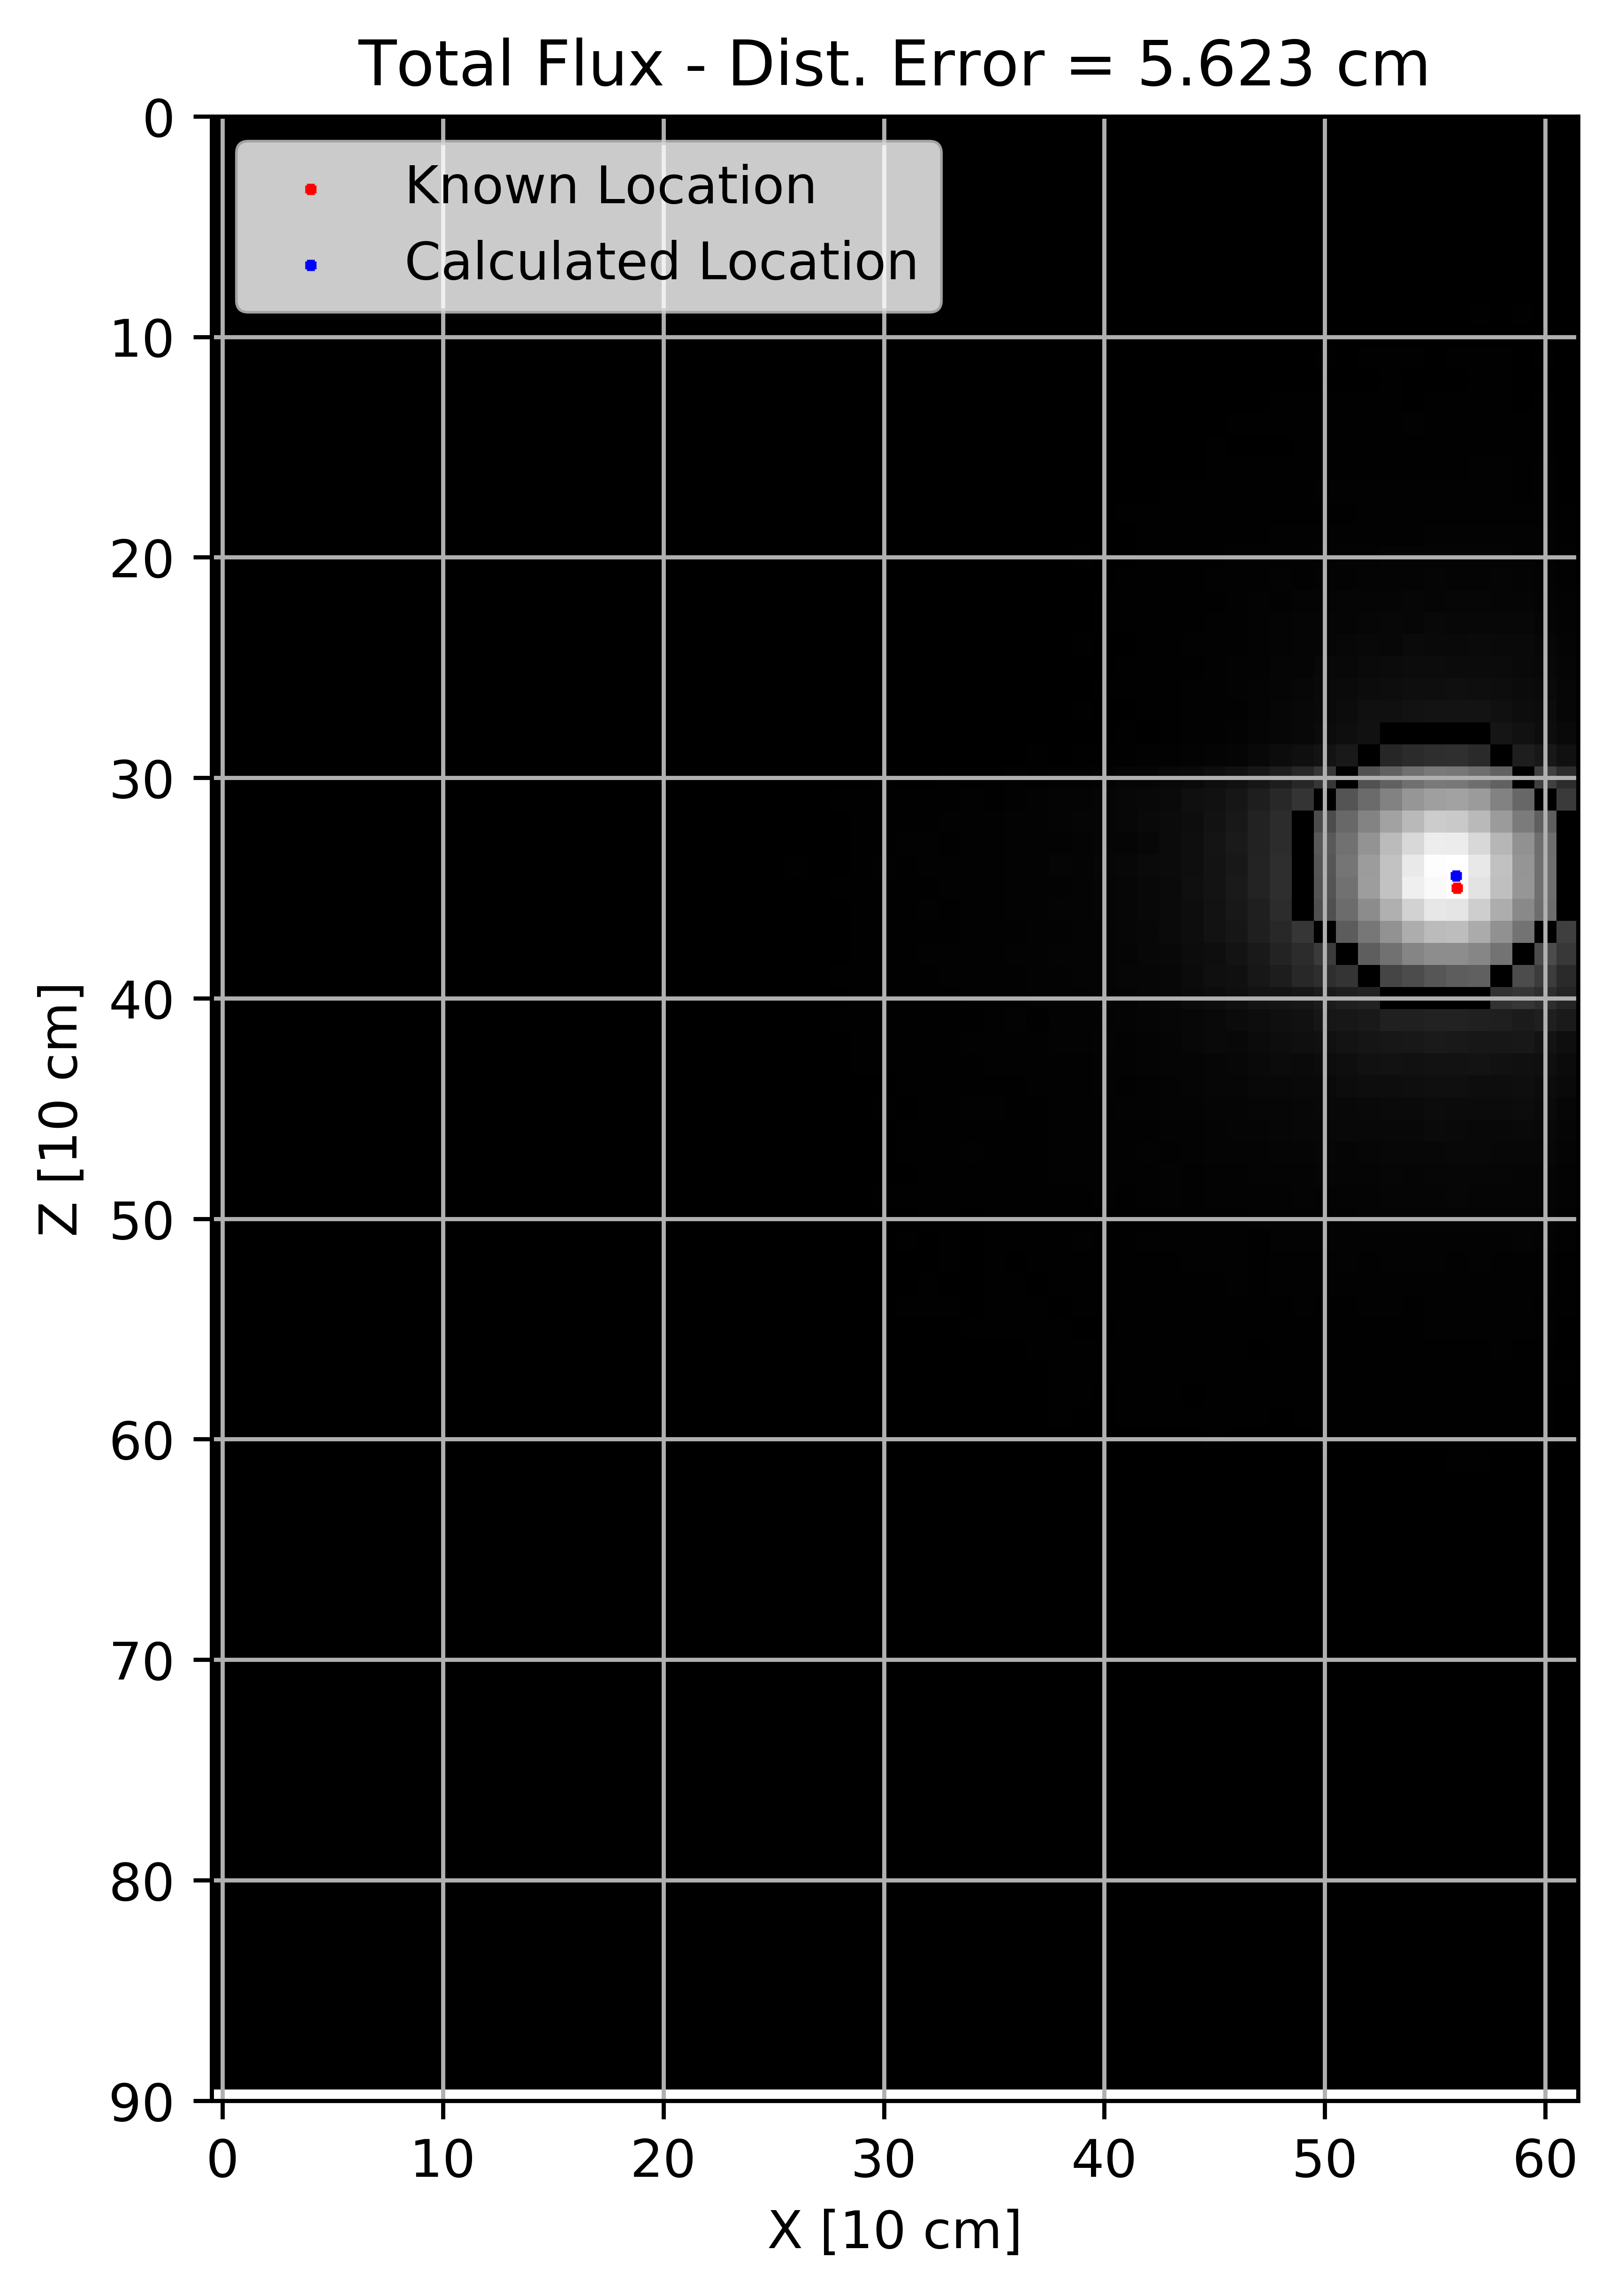
\includegraphics[width=1\linewidth]{images/2Cent_Total_2fl_Wall_S}
   \caption{}
   \label{fig:RanT2W}
\end{subfigure}
\begin{subfigure}[b]{0.15\textwidth}
   \centering
   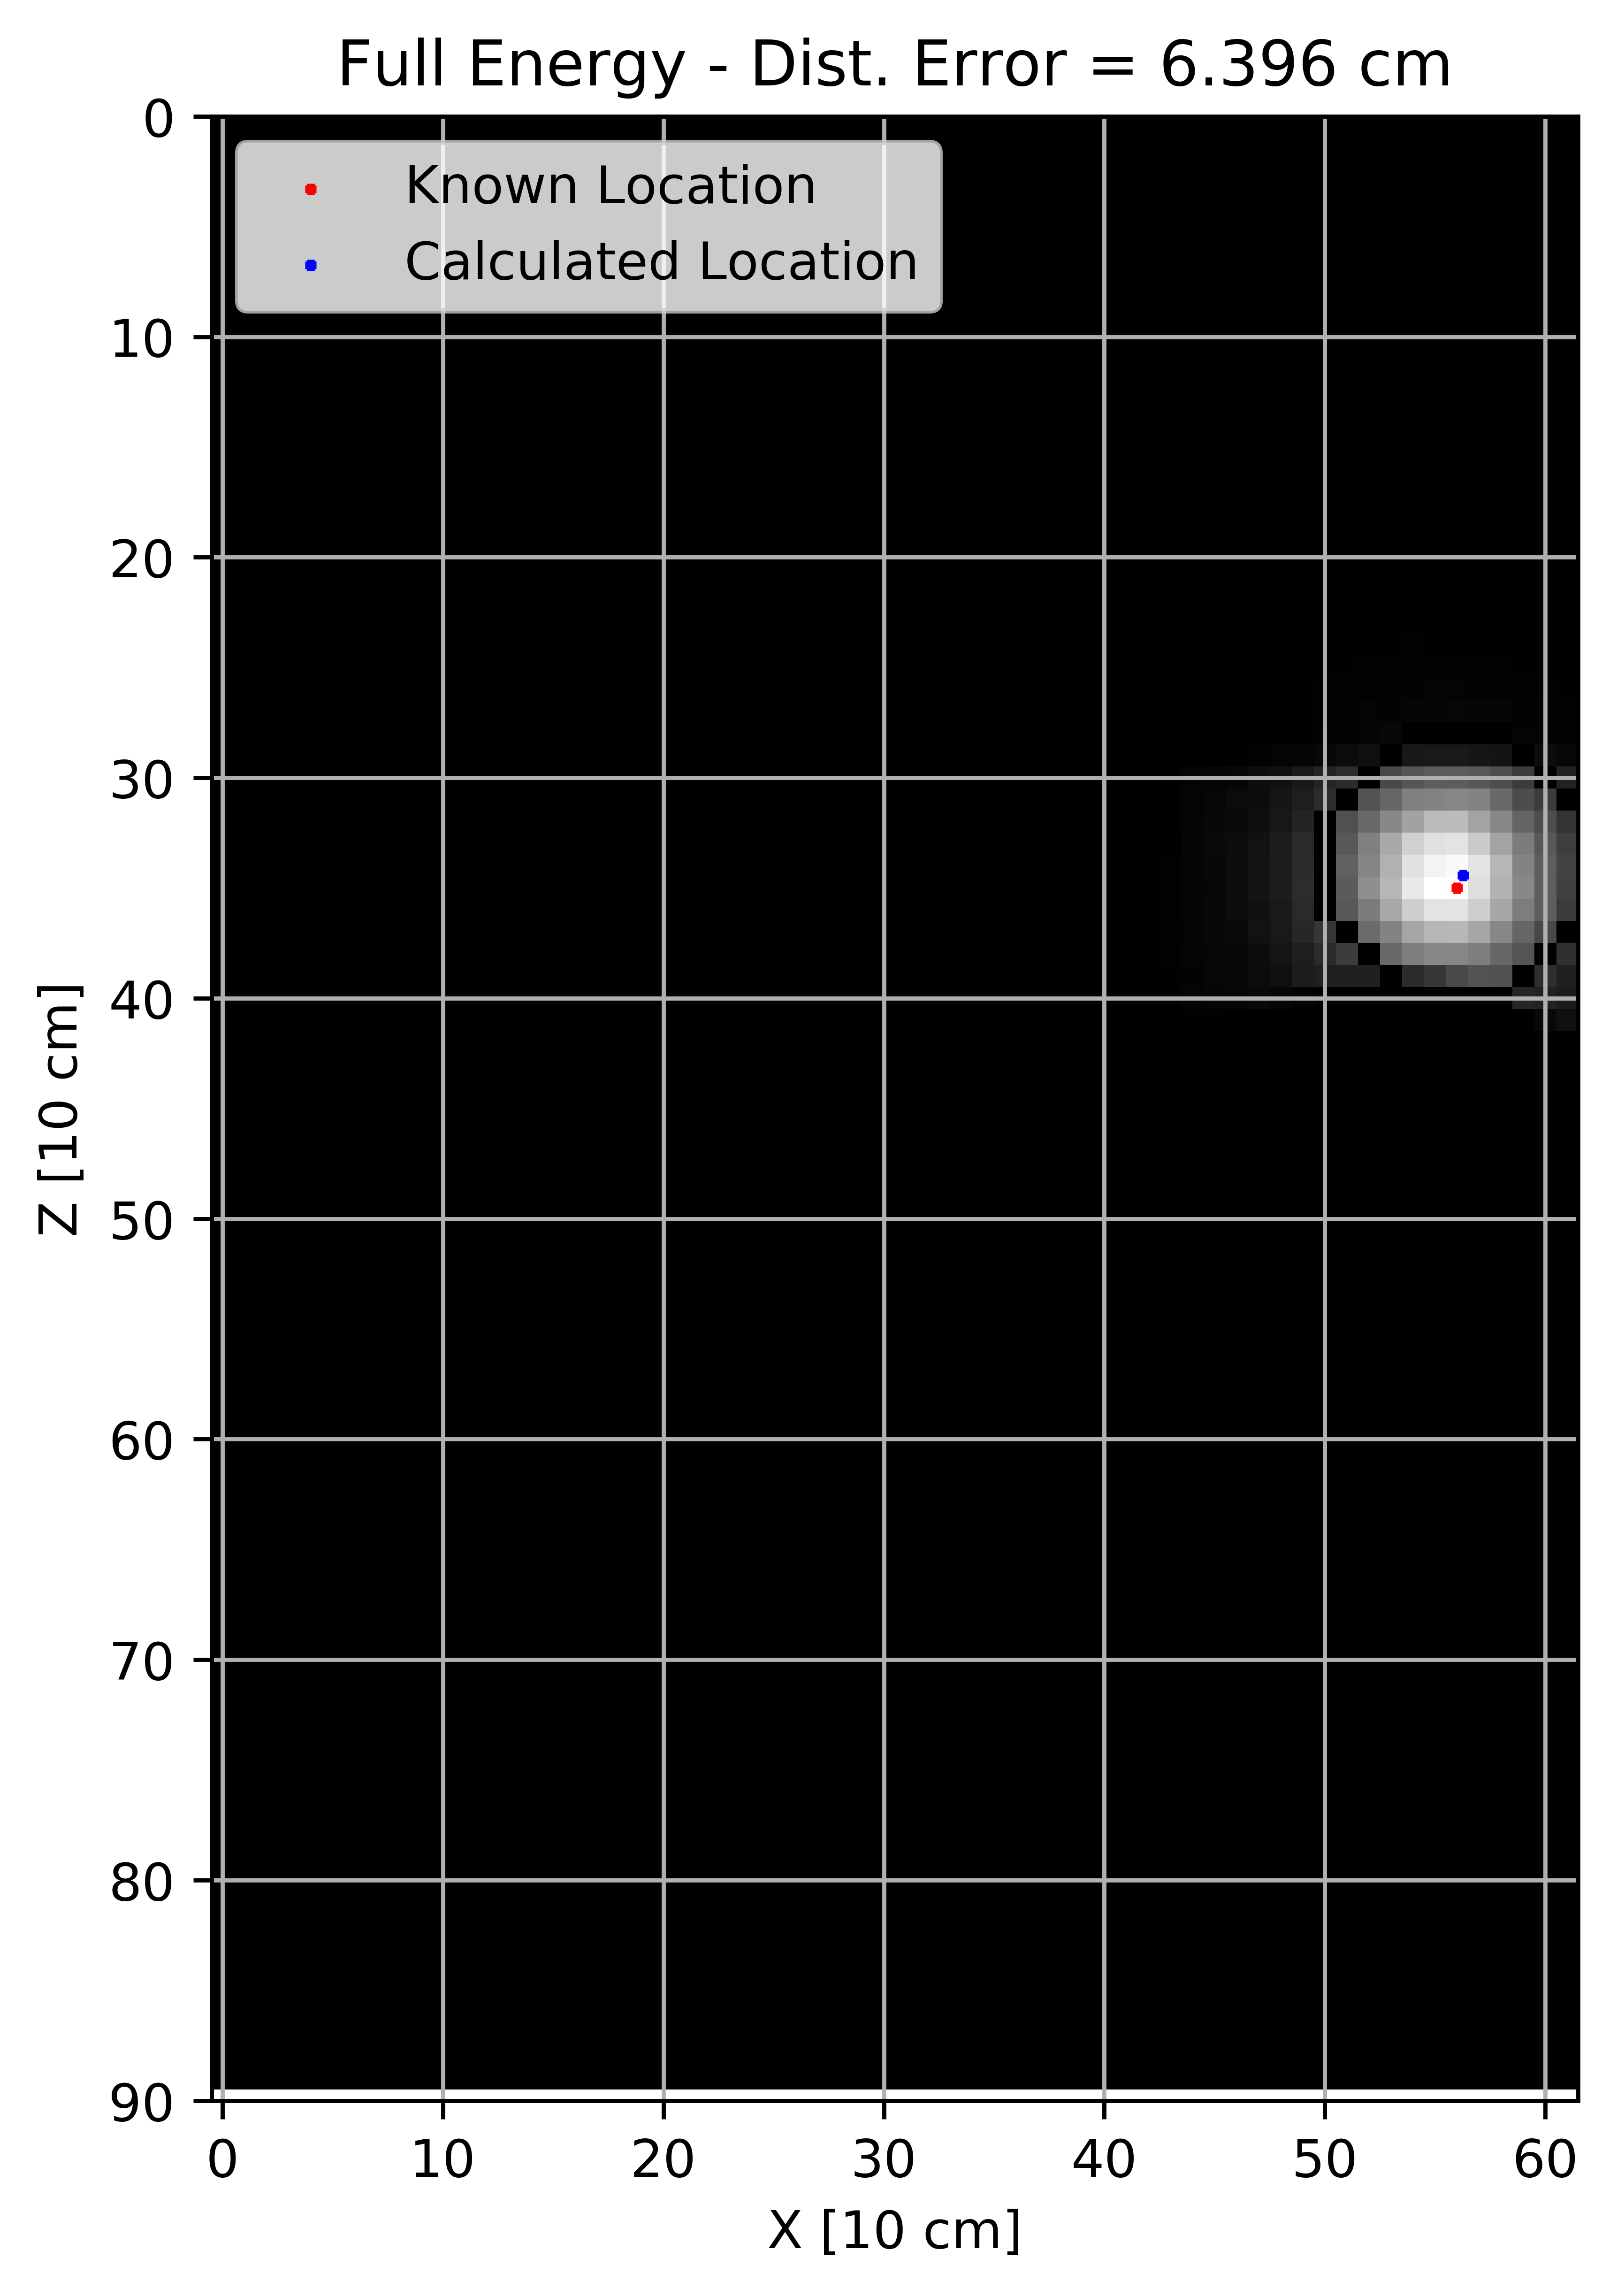
\includegraphics[width=1\linewidth]{images/2Cent_Full_2fl_Wall_S}
   \caption{}
   \label{fig:RanF2W}
\end{subfigure}
\begin{subfigure}[b]{0.15\textwidth}
   \centering
   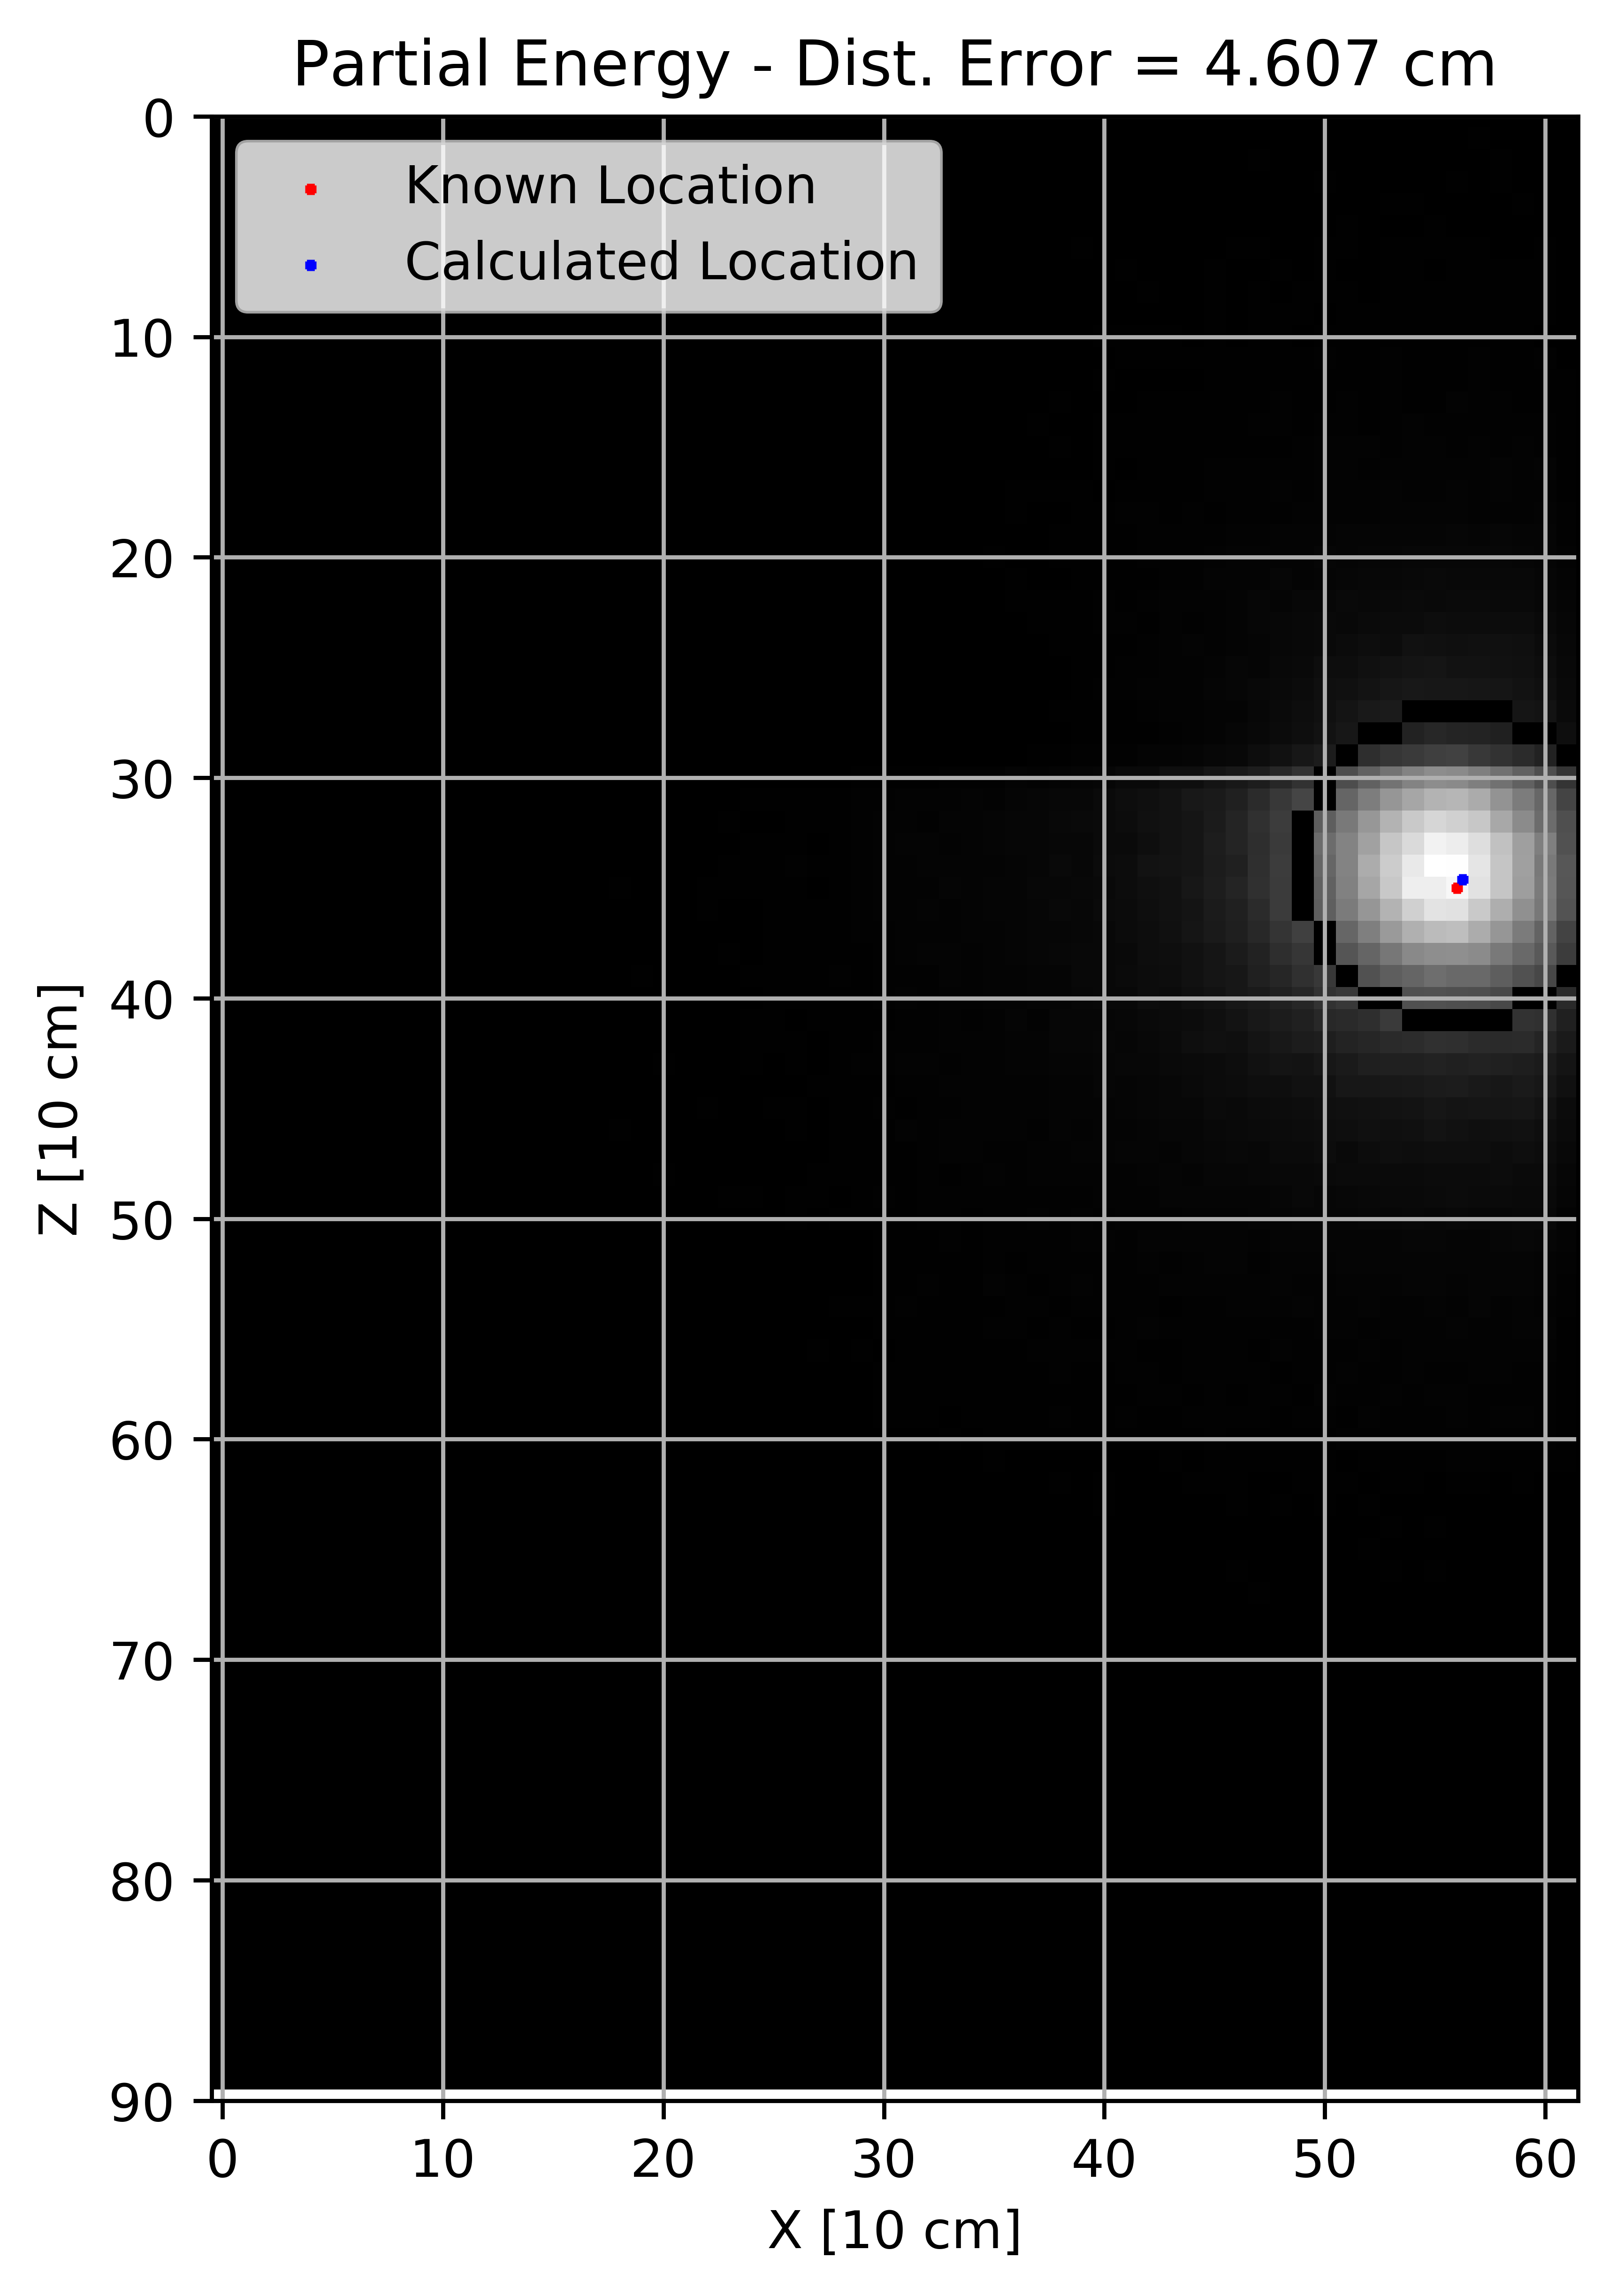
\includegraphics[width=1\linewidth]{images/2Cent_Part_2fl_Wall_S}
   \caption{}
   \label{fig:RanP2W}
\end{subfigure}
\caption{(a) Estimated source location using total flux from South. (b) Estimated source location using full energy flux from South. (c) Estimated source location using partial flux from South.}
\end{figure}

\begin{figure}[!htb]
\begin{subfigure}[b]{0.15\textwidth}
   \centering
   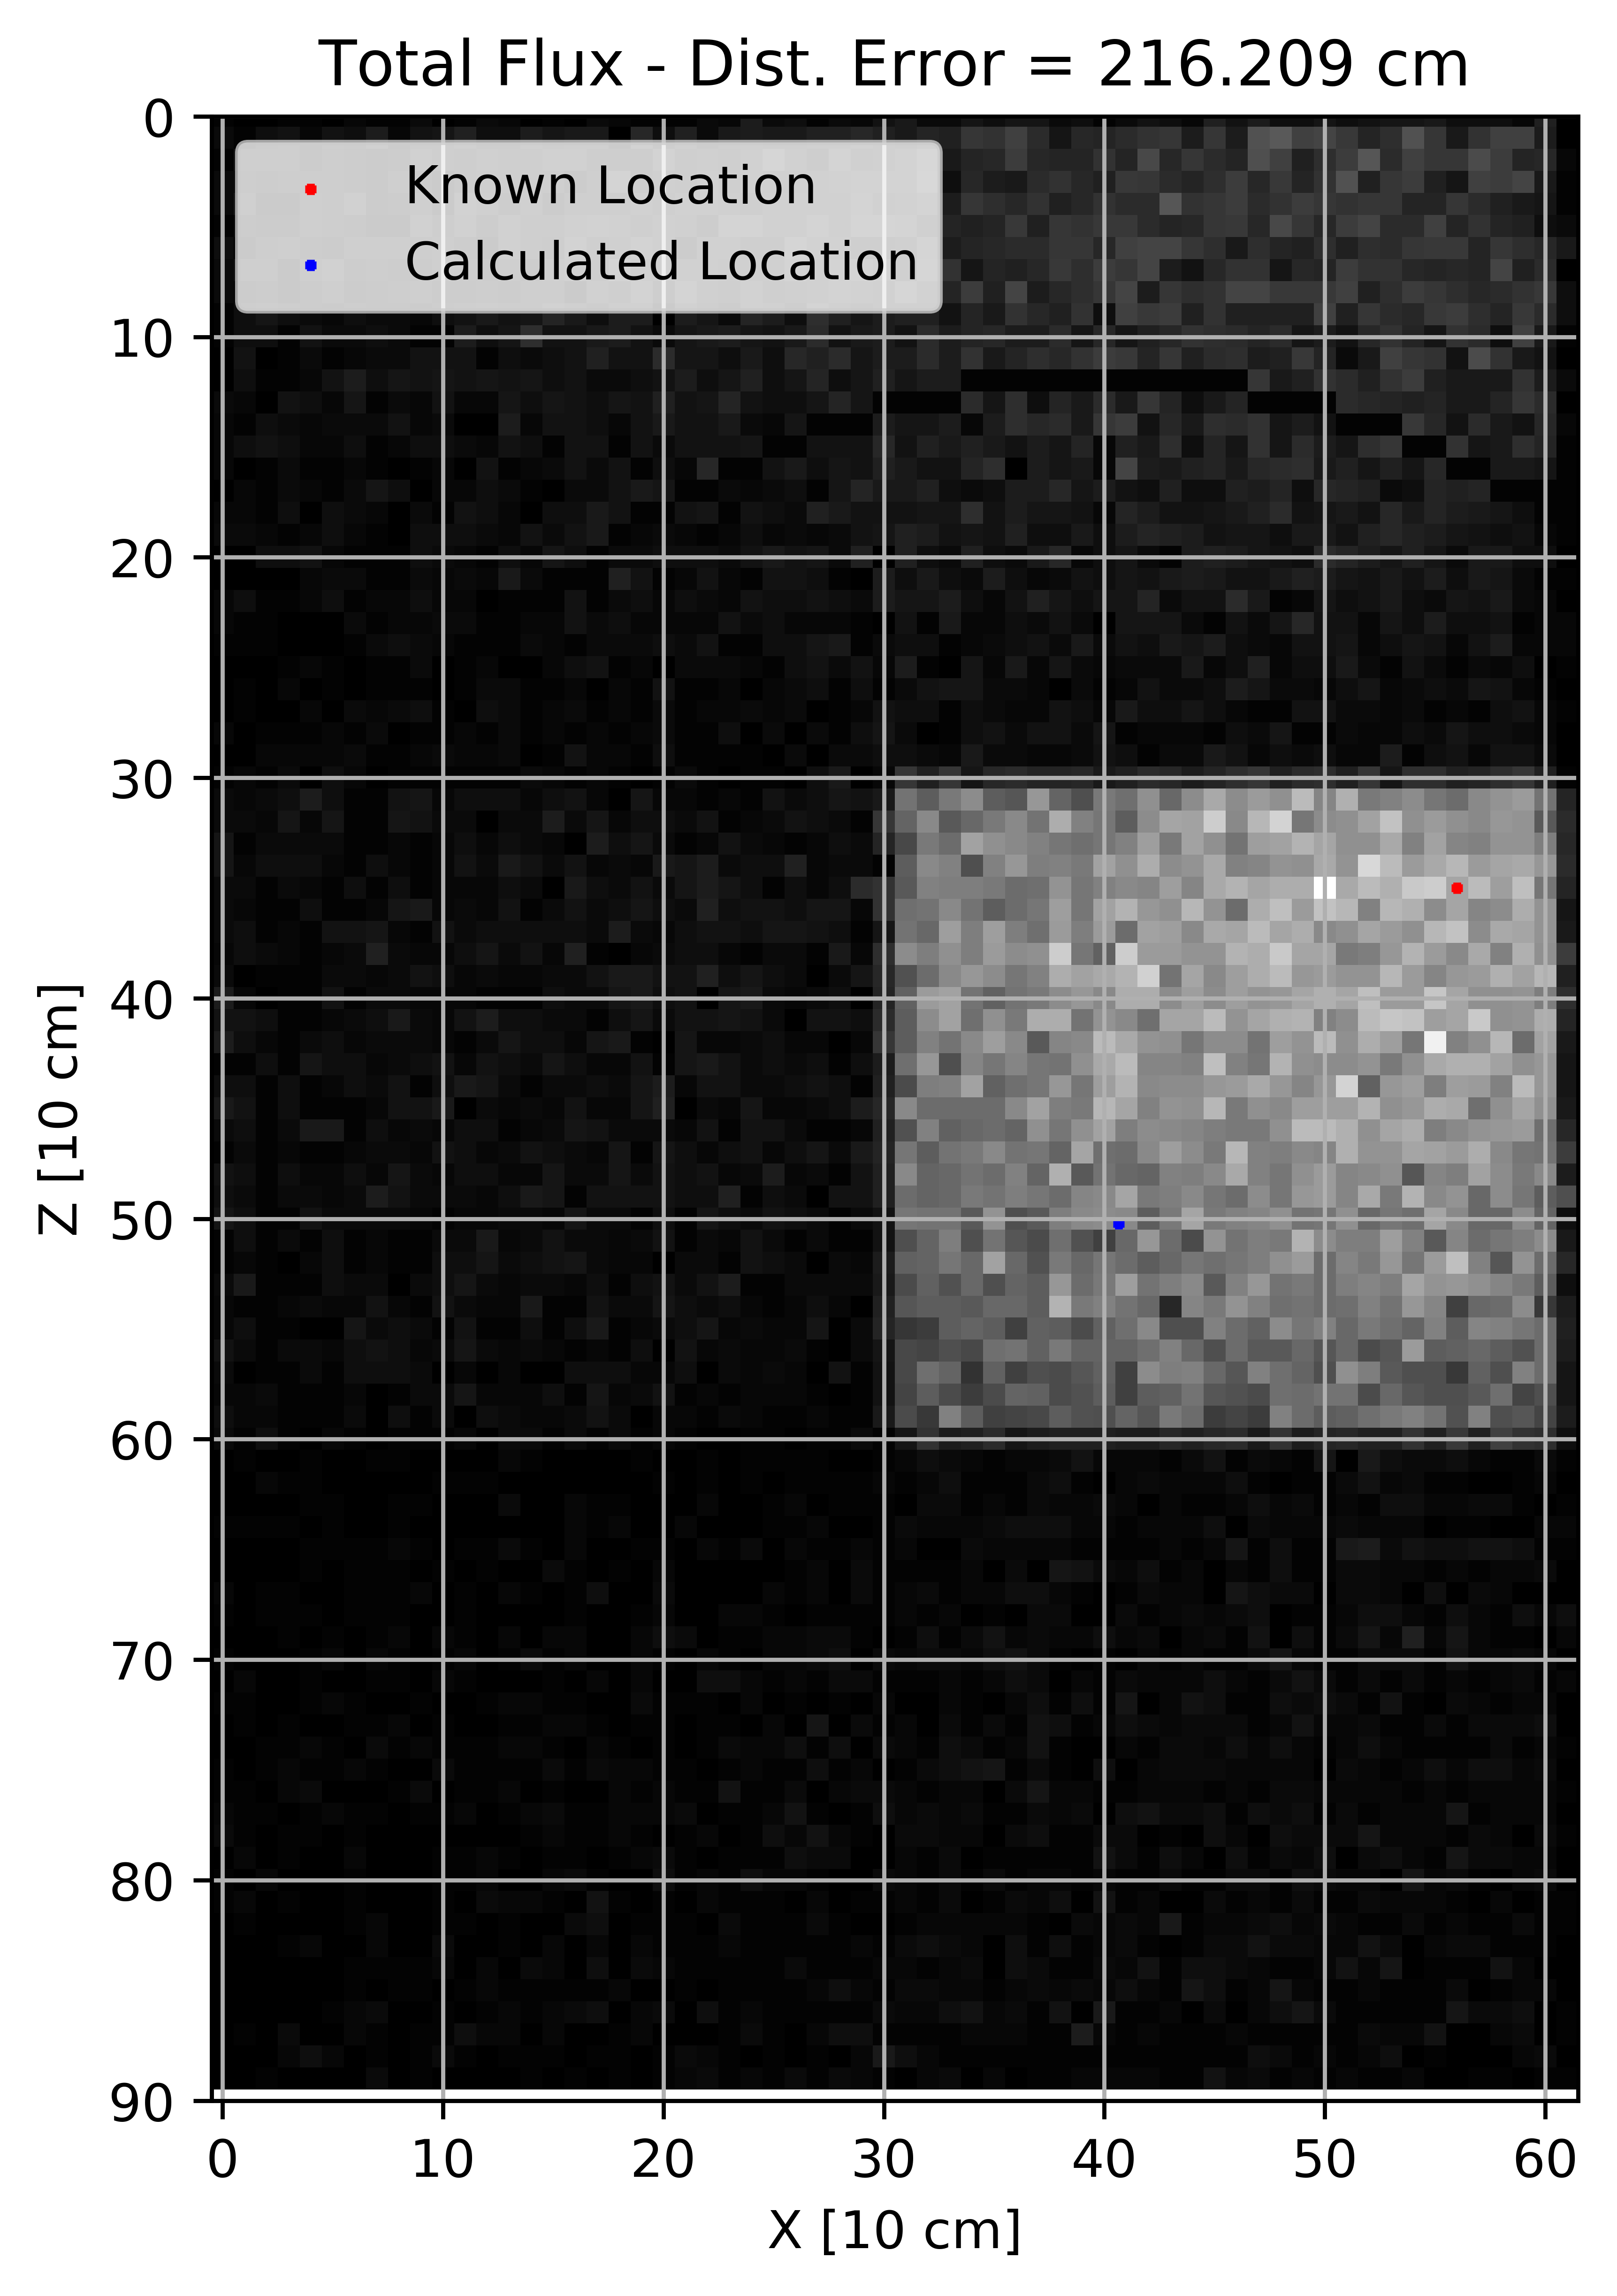
\includegraphics[width=1\linewidth]{images/2Cent_Total_2fl_Wall_N}
   \caption{}
   \label{fig:RanT2WN}
\end{subfigure}
\begin{subfigure}[b]{0.15\textwidth}
   \centering
   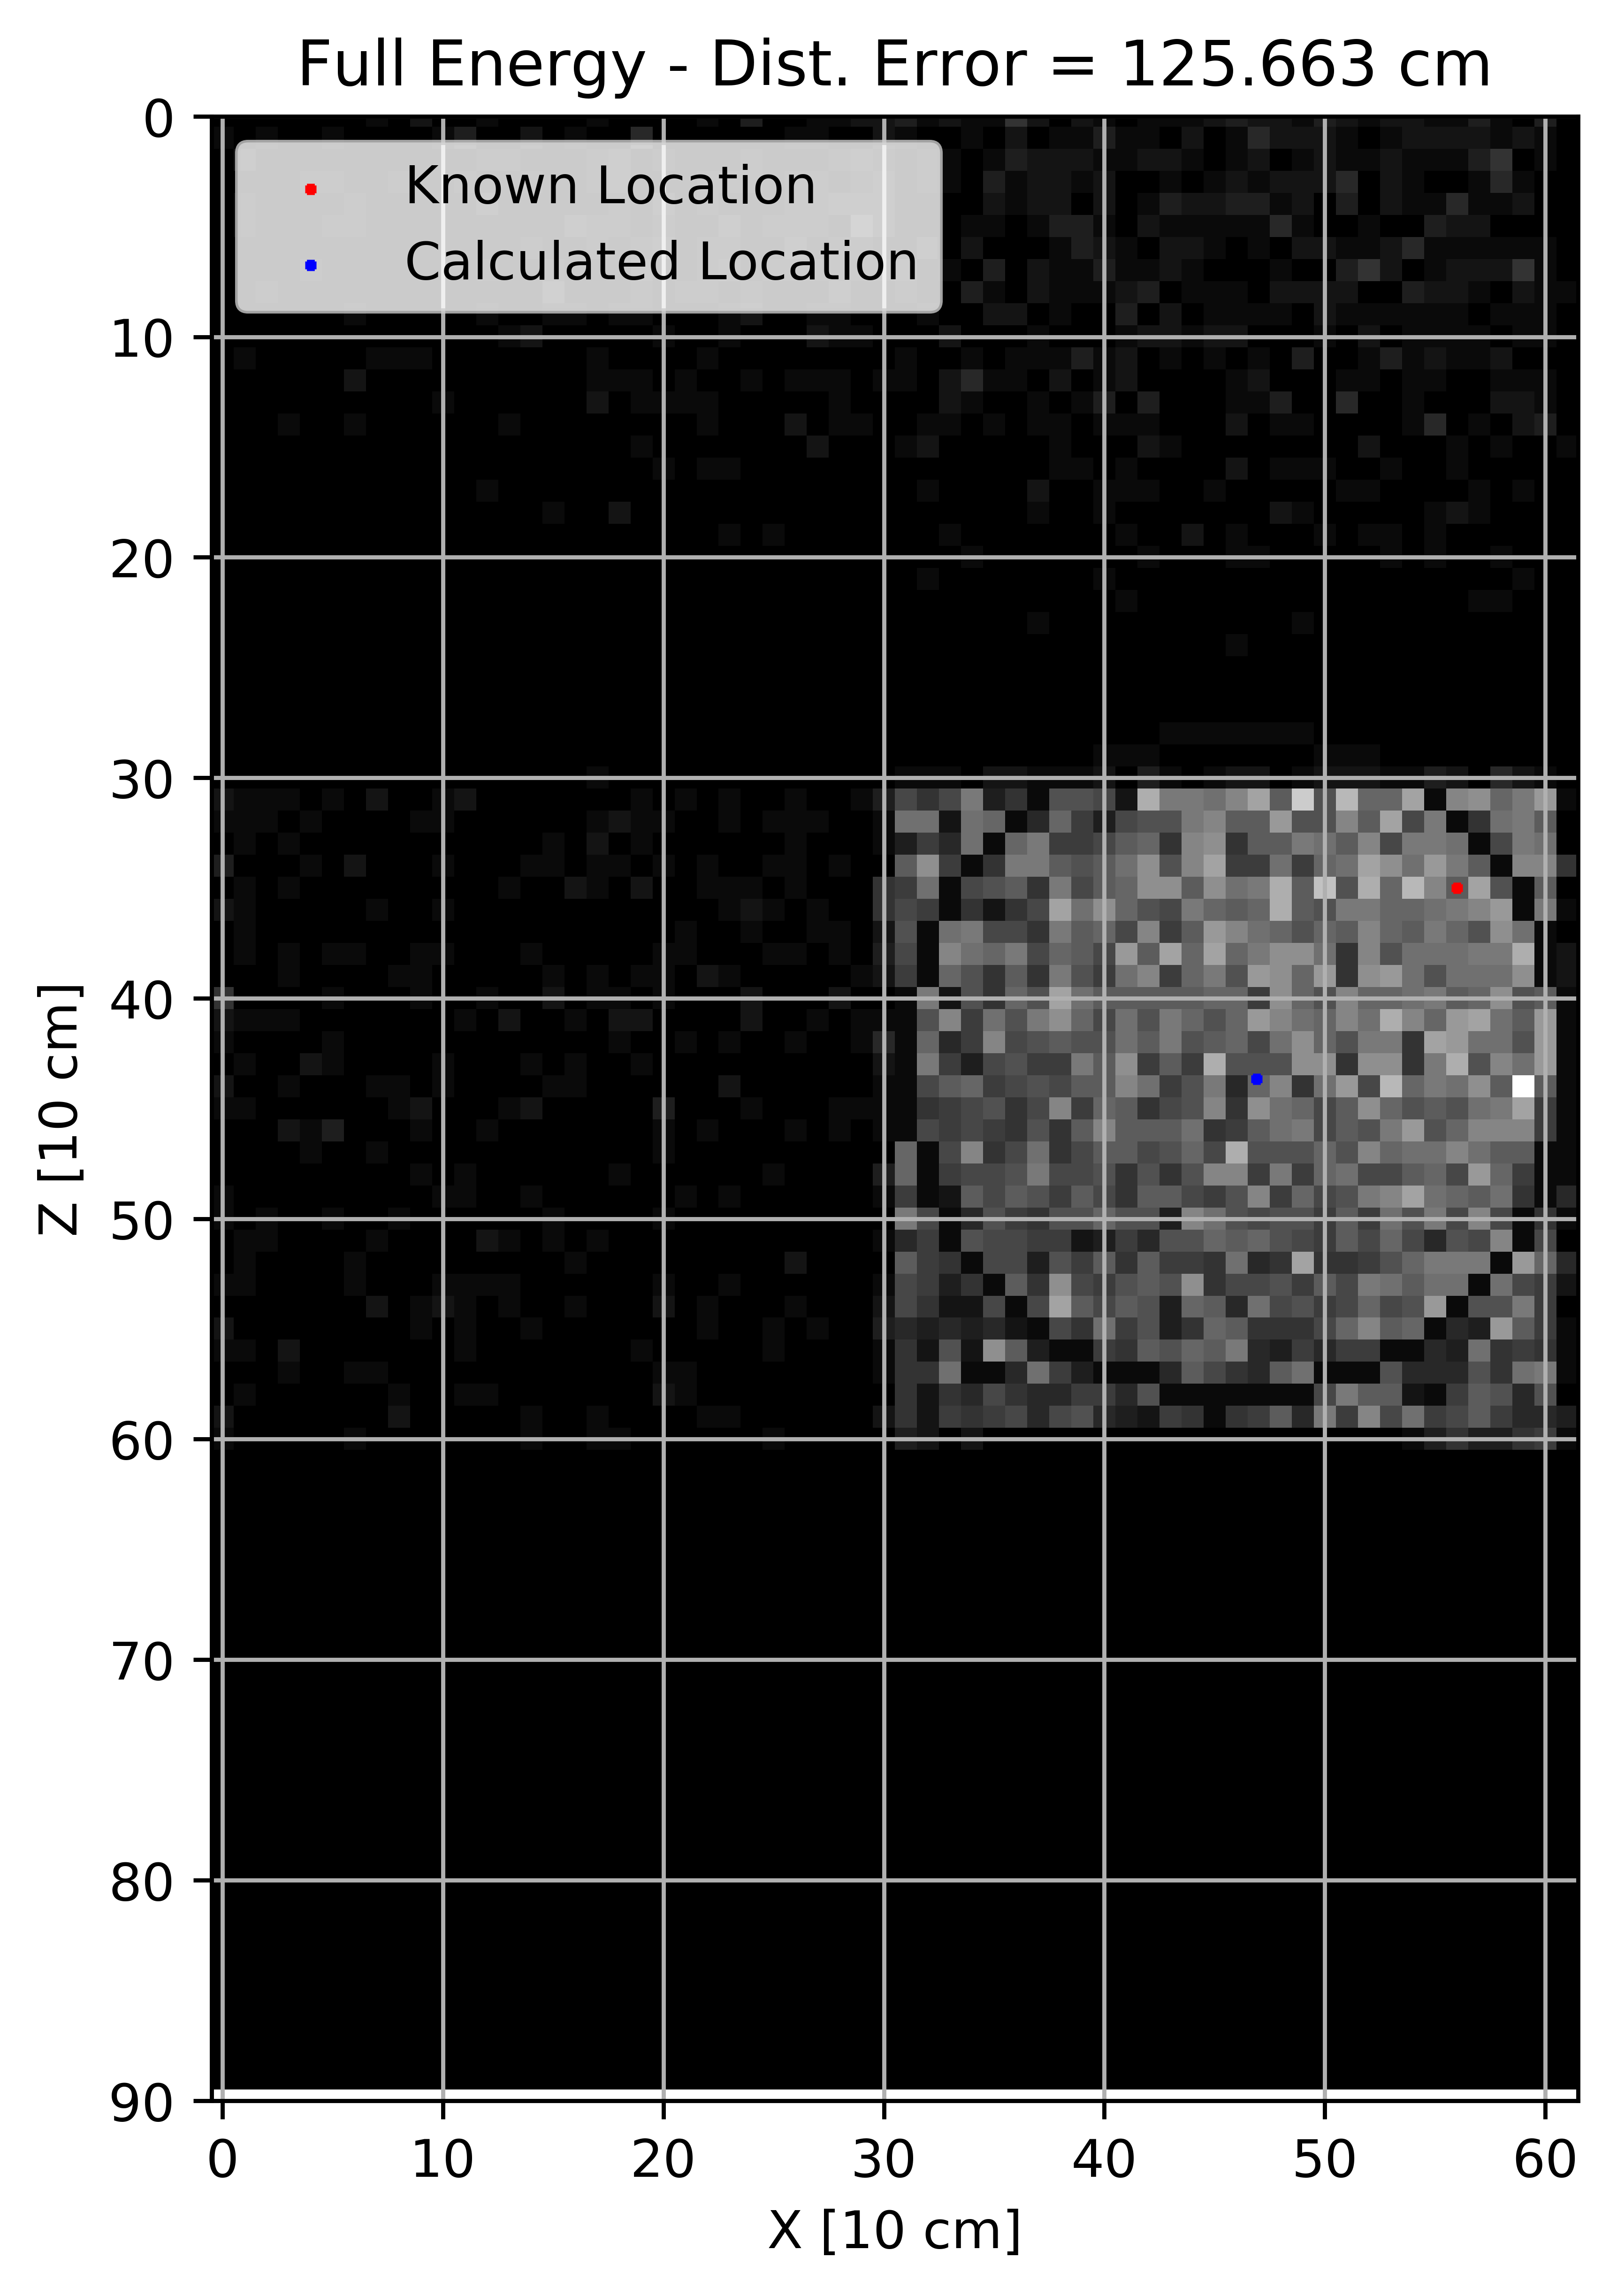
\includegraphics[width=1\linewidth]{images/2Cent_Full_2fl_Wall_N}
   \caption{}
   \label{fig:RanF2WN}
\end{subfigure}
\begin{subfigure}[b]{0.15\textwidth}
   \centering
   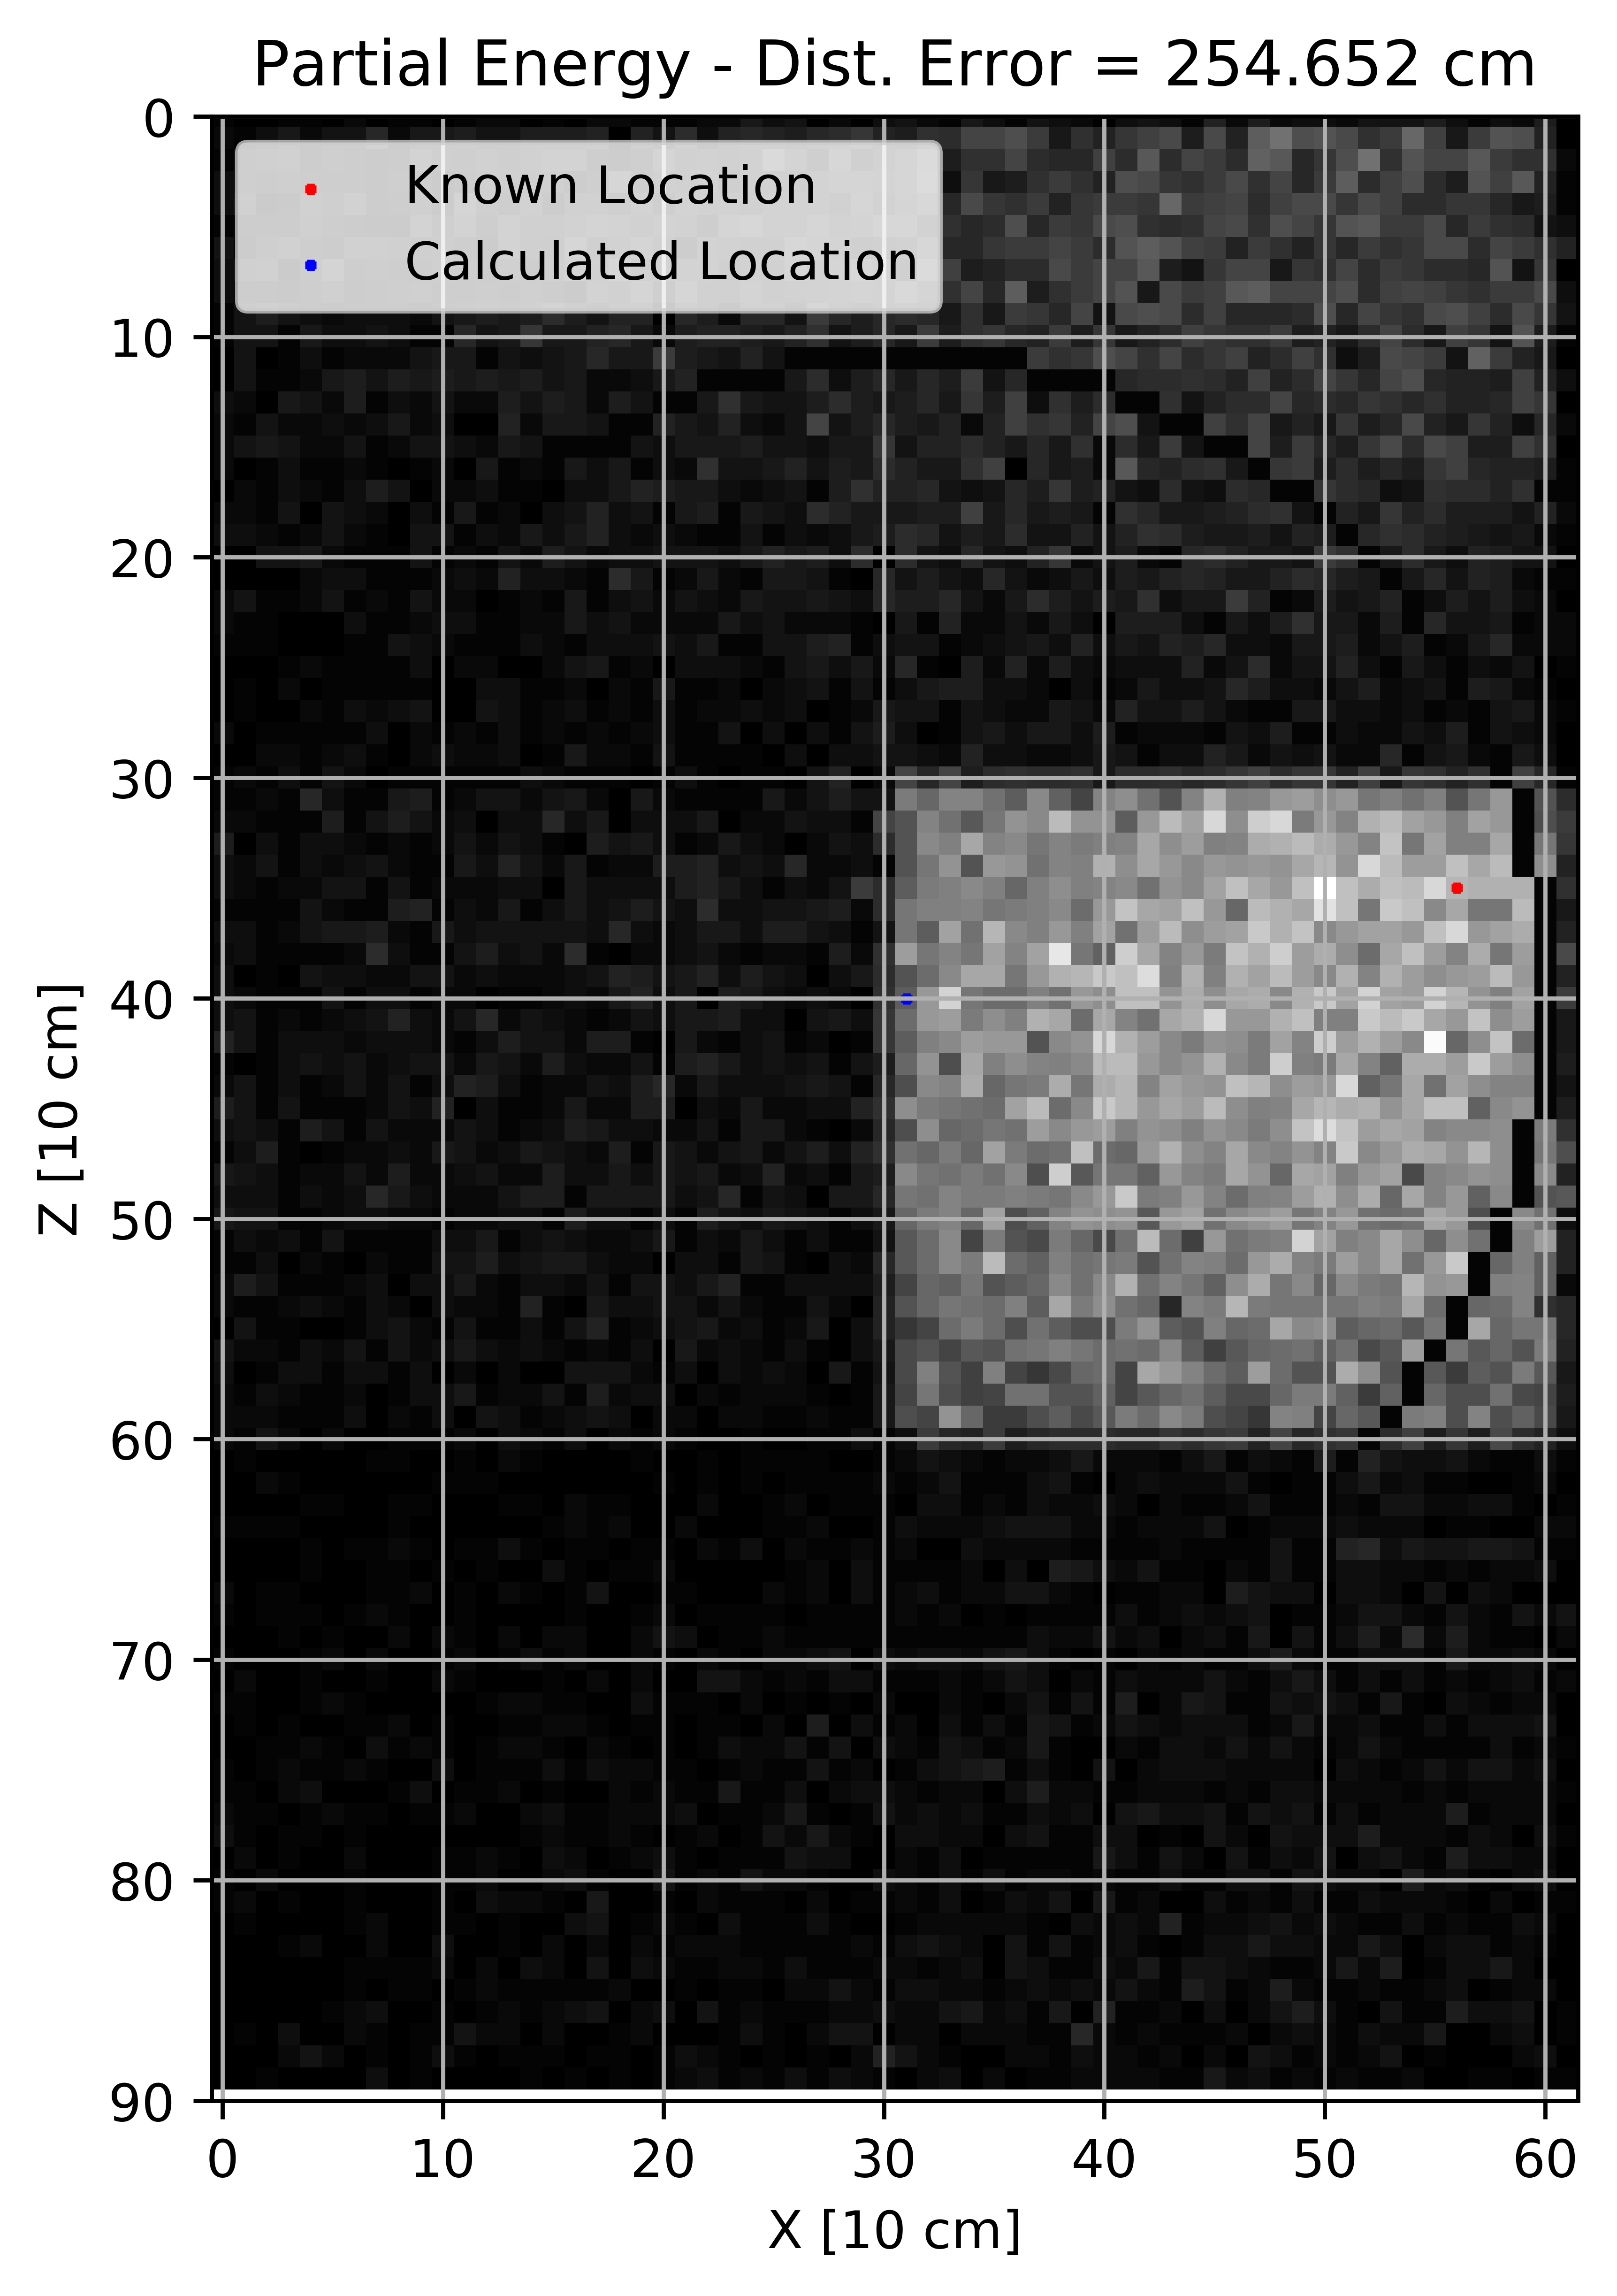
\includegraphics[width=1\linewidth]{images/2Cent_Part_2fl_Wall_N}
   \caption{}
   \label{fig:RanP2WN}
\end{subfigure}
\caption{(a) Estimated source location using total flux from North. (b) Estimated source location using full energy flux from North. (c) Estimated source location using partial flux from North.}
\end{figure}

\noindent Figs. \ref{fig:RanT2W}, \ref{fig:RanF2W}, and \ref{fig:RanP2W} all show an accuracy of less than 7 cm, this is particularly impressive given the detector distance from the source and 10 cm of concrete. However, Figs. \ref{fig:RanT2WN}, \ref{fig:RanF2WN}, and \ref{fig:RanP2WN} show how it can be hard to localize from the far side of the building and how the radial dispersion of total and partial flux lead to larger lateral error.
\\\\
\begin{table}[!htp]
 \caption{Error in Estimated Source Location}
  \begin{center}
    \begin{tabulary}{\columnwidth}{cccc}
      \hline
      Floor & Location & Response & Error [cm] \\ \hline
      1 & Central & Total & 165.76 \\
      1 & Central & Full E & 92.95\\
      1 & Central & Partial E & 173.09 \\
      1 & Middle & Total & 138.86 \\
      1 & Middle & Full E & 54.52 \\
      1 & Middle & Partial E & 100.95 \\
      1 & Wall & Total & 394.93 \\
      1 & Wall & Full E & 30.22 \\
      1 & Wall & Partial E & 354.67 \\
      2 & Central & Total & 134.64 \\
      2 & Central & Full E & 101.34 \\
      2 & Central & Partial E & 149.89 \\
      2 & Middle & Total & 36.30 \\
      2 & Middle & Full E & 79.29 \\
      2 & Middle & Partial E & 48.54 \\
      2 & Wall & Total & 316.12 \\
      2 & Wall & Full E & 7.43\\
      2 & Wall & Partial E & 51.54 \\
      3 & Central & Total & 89.33 \\
      3 & Central & Full E & 37.25 \\
      3 & Central & Partial E & 99.52 \\
      3 & Middle & Total & 36.14 \\
      3 & Middle & Full E & 23.86 \\
      3 & Middle & Partial E & 36.91 \\
      3 & Wall & Total & 361.73 \\
      3 & Wall & Full E & 36.40 \\
      3 & Wall & Partial E & 385.27 \\\hline
    \end{tabulary}
  \end{center}
  \label{table:error}
\end{table}

Table \ref{table:error} shows the location error for all nine simulations. In all but one scenario the gating on the peak energy yields a marked improvement over gross counts and partial energy counts. The best case estimated the source within 8 cm of its actual location. This level of fidelity, if provided to search and recovery personnel would dramatically reduce their exposure and risk.
